\section{Independent validation and measured performance}\label{sec:experiments}

\subsection{Protocol and limits of the evidence}

All oracle inputs are frozen exact face pairings and integer coordinate vectors. Reconstructing a triangulation from a current library simplification command could change labels, basis choices and runtime; the supplied JSON avoids that ambiguity. The inherited oracle corpus uses Regina's 7.4 API and contains 48 finite triangulations, 1,801 standard vertex surfaces and 617 quadrilateral vertex surfaces. The new optional live cross-checks used the installed Regina 7.4.1 wheel. The runtime producers and saved-certificate replay do not require Regina.

The corpus includes layered and capped solid tori, interior-vertex subdivisions, finite trefoil and figure-eight exteriors, and reducible torus-boundary controls involving $\mathbb{RP}^3$ and $S^2\times S^1$ summands. These are triangulation fixtures, not 48 distinct knots. General torus-boundary controls test hypotheses and failure modes; they do not establish diagram provenance.

The broad audit and controlled timing experiment are separate. The broad audit ran each method once per sector, in a fixed order, while other research work could be active. Its wall times are exploratory. Controlled timings ran after all CPU-heavy audit and test jobs had completed, used one warm-up and five measured repetitions, and shuffled method order using seed 20261009. The host exposed an AMD EPYC 9V74 processor and nine logical CPUs; Python was 3.12.14. Shared-host scheduling remained uncontrolled. Raw observations and the A/A controls are included; these small samples are not a statistical population study.

Each timed producer call includes its public validation and source-model construction. Independent replay is timed separately. Fixture generation, external oracle enumeration, JSON serialization and file I/O are outside the timed region. The old sector baseline answers the same positive-Euler existence query by Q-ray enumeration and early stopping; the new producer additionally constructs its arithmetic certificate. The ray comparison times both production and independent replay for the same supplied primitive meridian.

\subsection{Sector audit: complete agreements and coverage}

The audit selects every full singleton-type sector for fixtures with at most five tetrahedra, 64 seeded random full sectors for larger fixtures, and the occupied supports and full extensions of known standard/Q vertices, deduplicated. There are 7,314 resulting supplied-sector queries. Both standard and Q oracles are independently reduced to canonical vectors before testing positive Euler, preventing removed vertex links from becoming spurious witnesses.

\begin{center}\small
\begin{tabular}{@{}lrr@{}}
\toprule
Quantity & Anchors with reuse & Envelope first\\
\midrule
Negative sector decisions & 5,499 & 5,499\\
Positive sector decisions & 1,815 & 1,815\\
Independent Euler replays & 7,314 & 7,314\\
Caps, oracle disagreements or replay failures & 0 & 0\\
Anchor tuples tested & 64,694 & 32,979\\
LP calls, including preliminary envelopes & 20,192 & 19,777\\
Reused anchor duals & 44,502 & 20,516\\
Simplex pivots & 87,695 & 91,219\\
Compact envelope-only negative proofs & --- & 3,663\\
Summed compact certificate bytes & 6,051,458 & 3,700,579\\
\bottomrule
\end{tabular}
\end{center}

Every complete answer agrees with both complete frozen ray lists and with the preceding sector enumerator. Every positive basic Q-direction appears in the full frozen Q oracle. The 1,815 positive outputs represent 110 distinct fixture/coordinate vectors. Each strategy produced 273 independently verified disc outcomes, representing 48 distinct vectors across 44 fixture IDs. Repeated outputs from overlapping sectors are not counted as new knots or new surfaces.

The envelope's 3,663 compact negative proofs are useful, but another 1,836 genuinely negative sectors needed anchor fallback after a positive envelope result. Together with the explicit two-variable counterexample, this confirms why envelope positivity cannot be treated as a surface witness. Certificate byte totals include source digests, supports, positive coordinates and negative dual records, but exclude full triangulations, statistics and separate ray-disc proofs. The approximately 38.85\% reduction in these bytes does not imply fewer pivots: the envelope total is higher.

Coverage reaches two active vertex groups, 44 anchor tuples and nullity five. The nullity histogram is
\[
\begin{array}{c|rrrrrr}
d&0&1&2&3&4&5\\\hline
\text{sectors}&48&4087&1802&988&359&30.
\end{array}
\]
Thus this is a substantial exact regression corpus, but it is predominantly low-nullity and does not test an asymptotic high-nullity crossover.

\subsection{Controlled sector timings: a mixed result}

The controlled cases were selected before timing by fixture and polarity, then by decreasing nullity, decreasing active vertex count, decreasing support size, and lexicographic support. Fourteen strata are present among the eight predeclared fixtures. Table~\ref{tab:sectors} reports milliseconds. ``LP'' means the ordinary anchor strategy with certified reuse; ``Env.'' means envelope first.

\begin{table}[htbp]
\centering\small
\begin{tabularx}{\textwidth}{@{}Xrrcrrrrr@{}}
\toprule
Fixture & $t$ & $d$ & Sign & Old & LP & Replay & Env. & Replay \\
\midrule
Fibonacci layered torus & 10 & 4 & $-$ & 6.24 & 12.88 & 2.15 & 14.99 & 2.19 \\
Fibonacci layered torus & 10 & 1 & + & 8.44 & 7.93 & 0.48 & 12.93 & 0.47 \\
Boundary-cap torus & 6 & 2 & $-$ & 0.74 & 0.35 & 0.39 & 0.37 & 0.34 \\
Boundary-cap torus & 6 & 5 & + & 1.50 & 0.65 & 0.28 & 0.79 & 0.27 \\
Trefoil & 5 & 2 & $-$ & 1.10 & 2.57 & 0.62 & 3.12 & 0.67 \\
Trefoil, interior vertex & 8 & 3 & $-$ & 2.87 & 5.46 & 1.72 & 6.45 & 1.56 \\
Trefoil, interior vertex & 8 & 3 & + & 2.58 & 10.84 & 0.39 & 11.95 & 0.37 \\
Figure-eight & 10 & 4 & $-$ & 14.71 & 21.35 & 3.11 & 23.35 & 3.06 \\
Figure-eight, interior vertex & 13 & 5 & $-$ & 48.58 & 55.05 & 5.61 & 60.88 & 5.60 \\
Figure-eight, interior vertex & 13 & 5 & + & 23.29 & 163.69 & 0.66 & 169.09 & 0.61 \\
Torus $\#\mathbb{RP}^3$ & 5 & 3 & $-$ & 2.24 & 0.48 & 0.67 & 0.59 & 0.40 \\
Torus $\#\mathbb{RP}^3$ & 5 & 5 & + & 0.98 & 0.50 & 0.24 & 0.56 & 0.23 \\
Torus $\#(S^2\!\times S^1)$ & 7 & 4 & $-$ & 2.42 & 0.99 & 0.99 & 0.91 & 0.60 \\
Torus $\#(S^2\!\times S^1)$ & 7 & 4 & + & 2.39 & 2.18 & 0.36 & 2.22 & 0.35 \\
\bottomrule
\end{tabularx}

\caption{Complete sector producers and separate independent replay; medians of five repetitions, in milliseconds. Sign is canonical positive-Euler existence, not a knot verdict.}\label{tab:sectors}
\end{table}

The ordinary LP producer wins on several controls, including the capped positive case and the reducible negative torus control. It loses substantially on other cases: the positive 13-tetrahedron figure-eight interior fixture takes about 163.69 ms, against 23.29 ms for early-stopping enumeration. Across these 14 deliberately structured strata, the geometric mean of old/new producer ratios is 0.914 for anchors and 0.802 for envelope first. Values below one favor the old producer. These selected cases do not justify making LP the unconditional default.

The broader one-shot audit is also unfavorable to LP on this corpus: old production totals 15.44 s, anchor production 81.54 s with 8.88 s replay, and envelope production 81.84 s with 6.19 s replay. These totals are disclosed as exploratory, not mixed with the controlled observations. They show why a polynomial reduction in a parameter is not itself an implementation speedup at the tested sizes.

The A/A sector control compares two calls to the identical old implementation under randomized ordering. Ratios range from 0.918 to 1.188 across strata. Consequently small percentage differences in submillisecond cases should not be overinterpreted. The large positive-figure-eight regression and the ray-path gains below are much larger effects, but still apply only to their measured queries.

\subsection{Primitive-ray disc validation and performance}

The short endpoint was compared against the essential-disc labels of all 1,801 frozen standard vertices. It agrees on every case. All 117 positive certificates replay independently with the producer disabled; 585 mutations are rejected. Mutations alter the prime, source fingerprint, selected rank rows, boundary proof or primitive coordinates. The M\"obius-plus-link counterexample is a separate control demonstrating that rank is a necessary logical gate for this shortcut.

For timing, the earlier public \code{normal_compressing_disk_count} producer is called with certificate recording, followed by \code{verify_normal_disk_count_certificate}. The new path constructs and replays the primitive-ray proof on the exact same coordinates. Both paths certify existence of an essential disc; the older general API can additionally count disc components on inputs outside the new endpoint's domain.

\begin{table}[H]
\centering\small
\begin{tabular}{@{}rrrrrrrr@{}}
\toprule
$t$ & Bits & Old build & Old replay & Ray build & Ray replay & Ratio & Ray bytes \\
\midrule
4 & 3 & 0.95 & 0.75 & 0.48 & 0.26 & 2.24 & 226 \\
8 & 6 & 2.01 & 1.53 & 0.49 & 0.50 & 3.47 & 262 \\
16 & 11 & 5.21 & 3.36 & 0.92 & 0.84 & 4.88 & 334 \\
32 & 22 & 14.66 & 7.31 & 1.73 & 1.91 & 6.17 & 521 \\
64 & 44 & 50.71 & 22.17 & 3.81 & 3.57 & 9.92 & 905 \\
128 & 89 & 182.02 & 71.05 & 7.08 & 7.61 & 17.55 & 1,673 \\
\bottomrule
\end{tabular}

\caption{Primitive Fibonacci meridians: times in milliseconds. ``Bits'' is maximum coordinate bit length. Ratio is old/new median construction-plus-replay time, computed from paired sums rather than from the separately displayed medians.}\label{tab:rays}
\end{table}

At 128 tetrahedra, construction plus replay improves by a factor of 17.55. The compact serialized proof shrinks from 1,784,558 bytes to 1,673 bytes. Both size measurements exclude the separately supplied triangulation and input coordinate vector; the general certificate itself contains additional core coordinates and component history. This is a restricted primitive-ray improvement, not a claim about every normal vector or complete recognition time.

\begin{figure}[H]
\centering
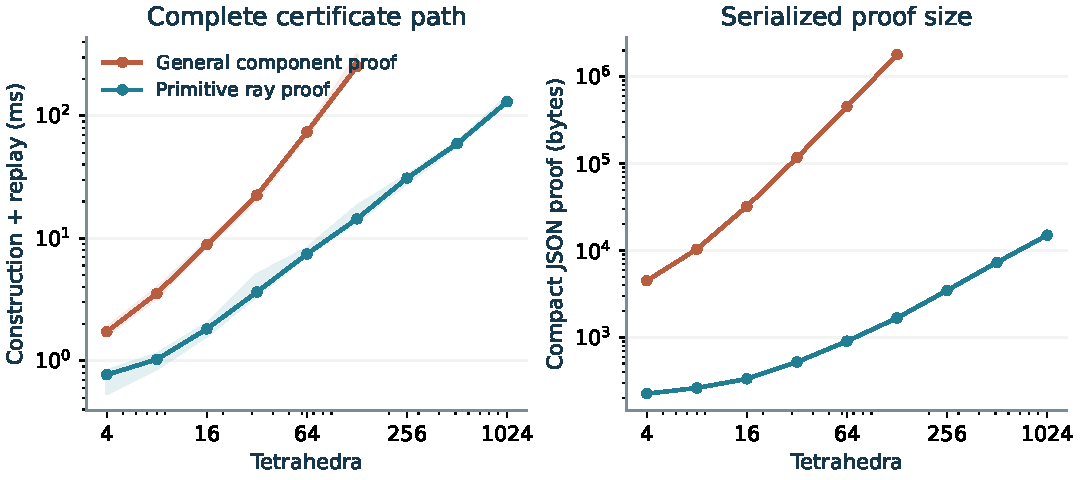
\includegraphics[width=\textwidth]{figures/primitive_ray_performance.pdf}
\caption{Full primitive-disc certificate paths on the Fibonacci family. Lines show medians; shaded time bands show the observed five-run range. The old path was measured only through 128 tetrahedra, so no later comparative speedup is asserted.}\label{fig:rays}
\end{figure}

\begin{center}\small
\begin{tabular}{@{}rrrrrr@{}}
\toprule
$t$ & Bits & Ray build (ms) & Replay (ms) & Rank operations & Proof bytes \\
\midrule
256 & 178 & 14.34 & 15.23 & 5,603 & 3,474 \\
512 & 355 & 29.42 & 28.79 & 11,235 & 7,314 \\
1024 & 711 & 66.58 & 65.69 & 22,499 & 14,994 \\
\bottomrule
\end{tabular}

\end{center}

At 1,024 tetrahedra the largest coordinate has 711 bits; the explicit normal-disc count is $F_{1029}-5$, far beyond a feasible expanded-sheet computation. The new producer and verifier take roughly 0.13 s combined. The recorded rank-operation counts at 256, 512 and 1,024 tetrahedra are 5,603, 11,235 and 22,499. These happen to follow $22t-29$ in this labeling; they are operation-counter observations, not a general fill-in theorem. The A/A general-ray control ratios range from 0.957 to 1.093.

\subsection{Propagation, caps and whole-suite correctness}

The exact standard-coordinate propagation search was run on the Fibonacci family through eight tetrahedra with branching prohibited. It returns the exact primitive meridian every time. It examines three original anchors before the first positive result, uses $4t-1$ LP calls and $t-1$ mandatory propagations, and makes no type guesses. The pivot counts are:
\[
\begin{array}{c|rrrrrrrr}
t&1&2&3&4&5&6&7&8\\\hline
\text{pivots}&7&59&163&354&702&1073&1688&2620.
\end{array}
\]
These measurements stop at the first witness. The all-anchor, arbitrary-$t$ zero-backdoor result comes from Section~\ref{sec:fibonacci}, not from extrapolating this table.

The literal five-tetrahedron trefoil fixture completes all 20 anchors negatively with 1,554 pivots, no branches and no mandatory updates. Its full negative certificate independently replays. A five-tetrahedron solid torus obtained by three $2$--$3$ moves needs one branch under the fixed policy. An empty permitted branch set is inconclusive; permitting tetrahedron 1 alone succeeds and exercises the fallback that branches inside $B$ even when the current conflict is elsewhere. These observations are deciding runs, not computed minima of the strong parameter.

The ten-tetrahedron figure-eight control exhausts its aggregate 10,000-pivot allowance after completing 21 of 40 anchors. It returns \status{INCONCLUSIVE} without a negative certificate. Its single exploratory run took about 79.48 s. This is an explicit limitation of the dense exact LP prototype, retained in the data rather than removed as an inconvenient benchmark. An interior-vertex positive-Euler control also fails the disc endpoint because its boundary class is zero, demonstrating the intended distinction between the two APIs.

The complete maintained-plus-new test discovery covers 1,287 unique successful test IDs. The initial sparse work layout omitted 14 pinned reference assets; this caused 13 import/data errors and no assertion failures. After restoring those unchanged assets, only the affected modules were rerun: 85 tests passed, with three previously successful tests repeated. The coverage record reconciles all 1,287 expected IDs with no missing or unexpected cases. Both the initial log and the recovery log are preserved. No production or test fixes were needed for that layout recovery.

Focused new tests include 240 exact random cones compared with exhaustive support-ray oracles; complete small-sector comparisons; interior and multiple boundary vertices; 20,000-bit coefficient transport; caps; cancellation; malformed and foreign proofs; omitted anchors and children; and verification with producer functions disabled. These checks support the implementation at the specified boundary. They do not replace the mathematical proofs or establish the missing global parameter theorem.
